\subsection{Second Isomorphism Theorem}
\begin{frame}
\frametitle{Second Isomorphism Theorem}
\begin{theorem}
	Let $H$ be a subgroup of $G$ and let $N$ be a normal subgroup of $G$.
	Then $(HN)/N \isomorphism H/(H\cap N)$.
\end{theorem}
\begin{lemma}
	Let $N$ be a normal subgroup of $G$ and let $\gamma : G \to G/N$ be the canonical homomorphism.
	Then the map $\phi$ from the set of normal subgroups of $G$ containing $N$ to the set of normal subgroup of $G/N$ given by $\phi(L) = \gamma[L]$ is one-to-one and onto.
\end{lemma}
\begin{lemma}
	If $N$ is a normal subgroup of $G$, then $H \cap N = HN = NH$.
	Furthermore, if $H$ is also normal in $G$, then $HN$ is normal in $G$.
\end{lemma}
\end{frame}

\begin{frame}
	\begin{figure}
		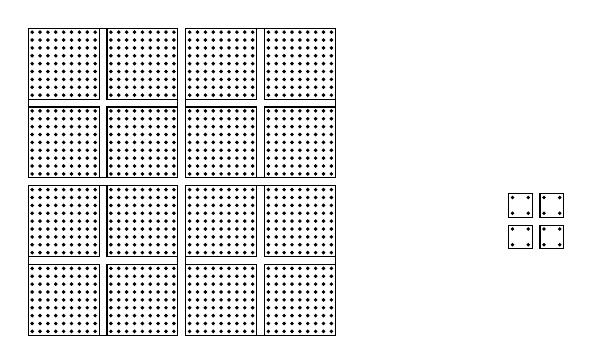
\begin{tikzpicture}
		%\draw[yellow,fill = yellow] (6.55,1.15) rectangle (6.85,1.45);
		%\draw[yellow,fill = yellow] (2.05,0.05) rectangle (3.95,1.95);
		%\draw[cyan,fill = cyan] (6.6,1.4) circle[radius=0.03];
		%\draw[cyan,fill = cyan] (2.05,1.05) rectangle (2.95,1.95);
		%\draw[red,fill = red] (2.7,1.2) circle[radius=0.03];

		%\draw node at (2,-1) {$G$};
		%\draw node at (2.9,1) {$g$};
		%\draw node at (6.5,0.5) {$G/H$};
		%\draw node at (0.5,0.5) {$H$};
		%\draw node at (2.5,1.5) {$gH$};
		%\draw node at (7.1,1.4) {$gH$};
		%\draw node at (1,1) {$K$};
		%\draw node at (8.5,0.5) {$G/K$};
		%\draw node at (9,1.25) {$gK$};
		%\draw node at (7.25,1.25) {$gK$};
		%\draw node at (3,1) {$gK$};
		%Group G
		%\draw<1-1> (0,0) rectangle (4,4);
		%coset division G/N
		\foreach \ii in {0,...,3}{
			\foreach \jj in {0,...,3}{
				\draw (0.05+\ii,0.05+\jj) rectangle (0.95+\ii,0.95+\jj);
			}}
		%coset division G/L
		\draw (0.05,0.05) rectangle (1.95,1.95);
		\draw (0.05,2.05) rectangle (1.95,3.95);
		\draw (2.05,0.05) rectangle (3.95,1.95);
		\draw (2.05,2.05) rectangle (3.95,3.95);
		%elements of G
		\foreach \ii in {0,...,3}{
			\foreach \jj in {0,...,3}{
				\foreach \kk in {1,...,9}{
					\foreach \ll in {1,...,9}{
						\draw[black,fill=black] (\ii.\kk,\jj.\ll) circle[radius=0.015];
			}}}}
		%Group G/N
		%\draw<4-4> (6,1) rectangle (7,2);
		%\coset division G/L
		\draw (6.15,1.15) rectangle (6.45,1.45);
		\draw (6.15,1.55) rectangle (6.45,1.85);
		\draw (6.55,1.15) rectangle (6.85,1.45);
		\draw (6.55,1.55) rectangle (6.85,1.85);
		%elements of G/N
		\foreach \ii in {2,4,6,8}{
			\foreach \jj in {2,4,6,8}{
				\draw[black,fill=black] (6.\ii,1.\jj) circle[radius=0.015];
			}}
		\end{tikzpicture}
	\end{figure}
\end{frame}
